\section{Discussion}
%%%%%%%%%%%%%%%%%%%%%%%%%%%%%%%%%%%%%%%%%%%%%%%%%%%%%%%%%%%%%%%%%%%%%%%%%%%%%%%%%%%%%%%%%
In this section we discuss our results and compare them with other results in the literature.
%%%%%%%%%%%%%%%%%%%%%%%%%%%%%%%%%%%%%%%%%%%%%%%%%%%%%%%%%%%%%%%%%%%%%%%%%%%%%%%%%%%%%%%%%
\subsubsection{Regge Ladders}
%%%%%%%%%%%%%%%%%%%%%%%%%%%%%%%%%%%%%%%%%%%%%%%%%%%%%%%%%%%%%%%%%%%%%%%%%%%%%%%%%%%%%%%%%
As we mentioned in chapter \ref{ChHist}, the Regge limit is a powerful tool for extracting the asymptotic behavior of perturbative amplitudes in the high-energy regime. For the elastic scattering event
\begin{equation}
	a(p_{1}) + b(p_{2}) \longrightarrow a(p_{3}) + b(p_{4}),
\end{equation}
the Regge limit is
\begin{equation}
	\frac{t}{m_{a} m_{b}} \rightarrow \infty \qquad \text{fixed } \frac{s}{m_{a} m_{b}} \qquad \text{fixed } \frac{m_{a}}{m_{b}} \label{RLimit}
\end{equation}
Lee \& Sawyer \cite{LeeSawyer} used the Regge limit to evaluate the series of ladder diagrams in the Bethe-Salpeter equation. This approach relies on second-quantized methods. For scalar $\varphi^{3}$ theory they found Regge behavior, with leading Regge trajectory function $R_{LS}(s)$ given by
\begin{equation}
	R_{LS}(s) = -1 + \frac{g^{2}}{8 \pi^{2}} \int\limits_{4m^{2}}^{\infty} \frac{\mathrm{d}\sigma}{(\sigma - s) \sqrt{\sigma (\sigma - 4 m^{2}) } } \label{LeeSaw1m}
\end{equation}
where we have kept their normalizations. After integrating over $\sigma$ we find
\begin{equation}
	R_{LS}(s) = -1 + \frac{g^{2}}{4 \pi^{2}} \frac{1}{\sqrt{s (4 m^{2} - s)}} \operatorname{arccos}{\left( \frac{2m^{2} - s}{2m^{2}} \right)}
\end{equation}
In order to visualize this function, we introduce the dimensionless variables
\begin{equation}
	U(s) \equiv \frac{s - 2m^{2}}{2m^{2}} \qquad \alpha \equiv \frac{g^{2}}{8\pi^{2} m^{2}}
\end{equation}
Then
\begin{equation}
	R_{LS}(s) = -1 + \frac{\alpha}{2} \left[ \frac{\arccos{\left(-U \right)}}{\sqrt{1 - U^{2}}} \right]
\end{equation}
Figures \ref{ReLSFig} and \ref{ImLSFig} contains the plots of $R_{LS}(s)$ as a function of $U$. Unlike $R_{\phi}(s)$ in figures \ref{ReRPhiFig} and \ref{ImRPhiFig}, the real part of $R_{LS}(s)$ is not constant in the region $s < (m_{a} - m_{b})^{2}$.

\begin{figure}
\centering
\includegraphics[scale=0.6]{Plots/ReLS2.pdf}
\caption[Real part of the Lee-Sawyer Regge trajectory function for massless $\phi^{3}$ theory]{Real part of $R_{LS}(U)$. The red lines correspond to $R_{LS} = 0, 1, 2$. We have used $\alpha = 0.5$.}
\label{ReLSFig}
\end{figure}

\begin{figure}
\centering
\includegraphics[scale=0.6]{Plots/ImLS2.pdf}
\caption[Imaginary part of the Lee-Sawyer Regge trajectory function for massless $\phi^{3}$ theory]{Imaginary part of $R_{LS}(U)$. The red lines correspond to $R_{LS} = 0, 1, 2$. We have used $\alpha = 0.5$.}
\label{ImLSFig}
\end{figure}

%\begin{figure}[h!]
%\centering
%\includegraphics[scale=0.403]{Figures/LeeSawyerRe.pdf} \qquad \includegraphics[scale=0.403]{Figures/LeeSawyerIm.pdf}
%\caption[The Lee-Sawyer Regge trajectory $R_{LS}(\xi_{s})$]{The real (left) and imaginary (right) parts of $R_{LS}(s)$. The red horizontal lines correspond to $J = 0, 1, 2$. We set the coupling parameter to $\alpha = 1$. Unlike $R_{\phi}(s)$, the real part of $R_{LS}(s)$ approaches $-1$ for negative large values of $s$.}
%\label{LeeSawyerPlot}
%\end{figure}

The expression (\ref{LeeSaw1m}) can be generalize to the case of two different masses:
\begin{equation}
\begin{split}
	R_{LS}(s) = {}& {-1} \\
	&+ \frac{g^{2}}{8 \pi^{2}} \int\limits_{(m_{a} + m_{b})^{2}}^{\infty} \frac{\mathrm{d}\sigma}{(\sigma - s) \sqrt{[\sigma - (m_{a} - m_{b})^{2}][\sigma - (m_{a} + m_{b})^{2}]}}
\end{split}
\end{equation}
After integration we find
\begin{equation}
	R_{LS}(s) = -1 + \frac{\beta}{2} \left[ \frac{\arccos{\left(-\xi_{s} \right)}}{\sqrt{1 - \xi^{2}_{s}}} \right]
\end{equation}
where
\begin{equation}
	\xi_{s} \equiv \frac{s - m_{a}^{2} - m_{b}^{2}}{2 m_{a} m_{b}}, \qquad \beta \equiv \frac{g^{2}}{8 \pi^{2} m_{a} m_{b}}
\end{equation}
The function $R_{LS}(s)$ shares the same asymptotic values with the trajectory function $R_{\phi}(s)$ that we found in \S\ref{SecMasslessSca4},
\begin{equation}
	R_{\phi}(s) = -1 + \frac{\alpha_{0}}{m_{a} m_{b}} \left[ \frac{1}{\sqrt{1 - \xi^{2}_{s}}} \right]
\end{equation}
Namely,
\begin{equation}
	\lim_{s \rightarrow \pm \infty} \operatorname{Re}{[R_{LS}(s)]} = -1, \qquad \lim_{s \rightarrow \pm \infty} \operatorname{Im}{[R_{LS}(s)]} = 0
\end{equation}
Just like $R_{\phi}$, the function $R_{LS}$ diverges at the threshold $s = (m_{a} + m_{b})^{2}$. However, unlike $R_{\phi}$, the function $R_{LS}$ does not diverge at the pseudothreshold $s = (m_{a} - m_{b})^{2}$. Indeed, $R_{LS}$ is real in the region $s < (m_{a} + m_{b})^{2}$, so for large values of the coupling some of the bound state energies will be real but negative. Unlike $R_{\phi}$, which is real only in the interval $(m_{a} - m_{b})^{2} < s < (m_{a} + m_{b})^{2}$, $R_{LS}$ is ``aware'' of the instabilities in scalar $\varphi^{3}$ theory and can include tachyonic states in the spectrum.

If $t$ is very large, then the conjugate length, the separation between the particles, is very small. Thus, the Regge limit (\ref{RLimit}) contracts ladder diagrams along the vertical direction (i.e. the $t$-channel). For example, at the one-loop level we have
\begin{equation}
	\vcenter{\hbox{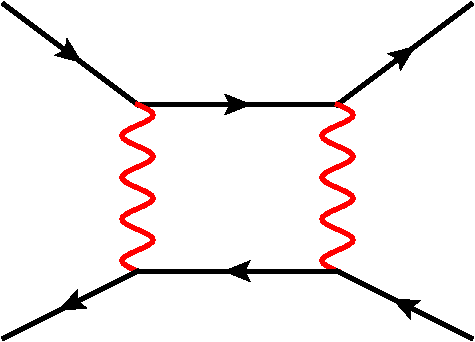
\includegraphics[scale=0.4]{Figures/1Box.pdf}}} \quad \longrightarrow \quad \vcenter{\hbox{\includegraphics[scale=0.4]{Figures/1Regge.pdf}}} \label{ReggeBox1}
\end{equation}
with the \textit{matter} propagators in the loop on the left living in $D$ dimensions, but those on the right living in $D - 2$ dimensions. The cubic interaction becomes a quartic interaction. Similarly, for the double box, we have
\begin{equation}
	\vcenter{\hbox{\includegraphics[scale=0.4]{Figures/2Box.pdf}}} \quad \longrightarrow \quad \vcenter{\hbox{\includegraphics[scale=0.4]{Figures/2Regge.pdf}}} \label{ReggeBox2}
\end{equation}
Indeed, the Regge trajectory $R_{LS}$ can be extracted from the \textit{exact} one-loop scalar box without taking the Regge limit. The exact one-loop amplitude can be found in \cite{PvN} (see \cite{tHVelt} for a more general result). It reads
\begin{equation}
	\mathcal{A}_{\text{box}} \sim \left( -\frac{2 \mu^{2}}{t} \right) H(s) \log{\left( -\frac{t}{2 \mu^{2}} \right)} \label{BoxAmp}
\end{equation}
where
\begin{equation}
	H(s) \equiv \int\limits_{(m_{a} + m_{b})^{2}}^{\infty} \frac{\mathrm{d}\sigma}{(\sigma - s) \sqrt{\Lambda(\sigma)}}
\end{equation}
with
\begin{equation}
	\Lambda(s) = [s - (m_{a} - m_{b})^{2}] [s - (m_{a} + m_{b})^{2}]
\end{equation}
The answer for the integral was given in \cite{PvN} as
\begin{equation}
	H(s) = \frac{1}{\sqrt{\Lambda(s)}} \log{\left( \frac{(m_{a} + m_{b})^{2} - s + \sqrt{\Lambda(s)}}{(m_{a} + m_{b})^{2} - s - \sqrt{\Lambda(s)}} \right)}
\end{equation}
which can be written as
\begin{equation}
	H(s) = \frac{1}{\sqrt{1 - \xi^{2}}} \arccos{\left( \sqrt{\frac{1 - \xi}{2}} \right)} = \frac{1}{2} \frac{\arccos(-\xi)}{\sqrt{1-\xi^{2}}}
\end{equation}
Hence, $R_{LS}(s) + 1$ is proportional to $H(s)$. The exact one-loop amplitude (\ref{BoxAmp}) has the same form as the one-loop amplitude (\ref{1Loop4D}) (modulo regularization), except that instead of $H(s)$ we have $\rho_{0}(s)$. Figures \ref{CompaReFig} and \ref{CompaImFig} have a graphical comparison.

\begin{figure}
\centering
\includegraphics[scale=0.6]{Plots/CompaRe2.pdf}
\caption[Comparison of the real part of $R_{LS}$ and $R_{\phi}$]{Real part of $R_{LS}(\xi)$ (magenta) and $R_{\phi}(\xi)$ (blue). The red lines correspond to $J = 0, 1, 2$. We have used $\alpha = 0.5$.}
\label{CompaReFig}
\end{figure}

\begin{figure}
\centering
\includegraphics[scale=0.6]{Plots/CompaIm2.pdf}
\caption[Comparison of the imaginary part of $R_{LS}$ and $R_{\phi}$]{Imaginary part of $R_{LS}(\xi)$ (magenta) and $R_{\phi}(\xi)$ (blue). The red lines correspond to $J = 0, 1, 2$. We have used $\alpha = 0.5$.}
\label{CompaImFig}
\end{figure}
%%%%%%%%%%%%%%%%%%%%%%%%%%%%%%%%%%%%%%%%%%%%%%%%%%%%%%%%%%%%%%%%%%%%%%%%%%%%%%%%%%%%%%%%%
\subsubsection{Eikonal Ladders}
%%%%%%%%%%%%%%%%%%%%%%%%%%%%%%%%%%%%%%%%%%%%%%%%%%%%%%%%%%%%%%%%%%%%%%%%%%%%%%%%%%%%%%%%%
All of our results were obtained from first-quantized path integrals in the eikonal JWKB approximation. Since we have ignored self-interactions, the only interaction terms in the (exact) quantum path integrals are two-body interactions. The quantum path integrals have a factor of the form
\begin{equation}
	{-1} + \exp{(i S_{2}^{F})} = i S_{2}^{F} + \frac{1}{2!} (i S_{2}^{F})^{2} + \frac{1}{3!} (i S_{2}^{F})^{3} + \ldots \label{LadderSeries}
\end{equation}
with $S_{2}^{F}$ being either of (\ref{S2Sca}), (\ref{S2Vec}), (\ref{Sh}) or (\ref{S2ScaM}). In order to be explicit, let us consider the two-body interaction from the massless scalar exchange. At lowest order, we have
\begin{equation}
	i S_{2}^{\phi} = i g_{0}^{2} \int \int \mathrm{d}\tau \mathrm{d}\sigma \, G_{0}[q_{a}(\tau) | q_{b}(\sigma)]
\end{equation}
This contribution can be interpreted as a tree level diagram: it corresponds to connecting a point in the worldline of particle $a$ to a point in the worldline of particle $b$ with a massless scalar propagator $G_{0}$. The integration over $\tau$ and $\sigma$ corresponds to summing over all pairs of points. The next order is
\begin{equation}
\begin{split}
	\frac{1}{2!} (i S_{2}^{\phi})^{2} = \frac{1}{2!} (i g_{0}^{2})^{2} \int \int \mathrm{d}\tau_{1} \mathrm{d} \sigma_{1} \int \int \mathrm{d} \tau_{2} \mathrm{d} \sigma_{2} \, {}& G_{0}[q_{a}(\tau_{1}) | q_{b}(\sigma_{1})] \\
	&\times G_{0}[q_{a}(\tau_{2}) | q_{b}(\sigma_{2})]
\end{split}
\end{equation}
For some values of $(\tau_{1}, \sigma_{1})$ and $(\tau_{2}, \sigma_{2})$ this contribution can be interpreted as a one-loop box diagram, but for other values it can be interpreted as a one-loop \textit{crossed} box diagram. Similar remarks hold for higher-order contributions. Thus, (\ref{LadderSeries}) can be interpreted as a first-quantized analog of the sum of ladder and crossed ladder diagrams.

In the eikonal JWKB approximation we evaluate $S_{2}^{\phi}$ and obtain $\Sigma_{2}^{\phi}$,
\begin{equation}
	\Sigma_{2}^{\phi} \approx -i \alpha_{0} \rho_{0} \Gamma\left( \frac{D - 4}{2} \right) \left(\frac{2}{\mu^{2} B_{12}^{2}} \right)^{(D - 4)/2}
\end{equation}
which is proportional to a massless scalar propagator in $D - 2$ dimensions. Thus, instead of the contraction (\ref{ReggeBox1}), we have
\begin{equation}
	\vcenter{\hbox{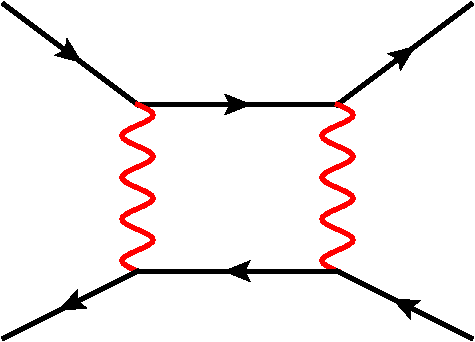
\includegraphics[scale=0.4]{Figures/1Box.pdf}}} \quad \longrightarrow \quad \vcenter{\hbox{\includegraphics[scale=0.4]{Figures/1Eikonal.pdf}}}
\end{equation}
and similarly for the double box in (\ref{ReggeBox2}):
\begin{equation}
	\vcenter{\hbox{\includegraphics[scale=0.4]{Figures/2Box.pdf}}} \quad \longrightarrow \quad \vcenter{\hbox{\includegraphics[scale=0.4]{Figures/2Eikonal.pdf}}}
\end{equation}
We see that the eikonal JWKB approximation contracts the ladder diagrams along the horizontal direction (i.e. either the $s$-channel or $u$-channel, since they are eikonal-equivalent because of $s + u = 2m_{a}^{2} + 2m_{b}^{2}$). However, these ``ladder diagrams'' are just schematic and do not correspond directly to (second-quantized) ladder diagrams since they come from a quantum mechanical path integral.

The work of Abarbanel \& Itzykson \cite{AbarbItzyk} has the same spirit as our work. Their functional derivative technique is equivalent to coupling the particles to an external field, integrating over this field, and then dropping the self-interactions. However, they push their approximations too far into the high-energy regime and reach a result (their equation 11) that is equivalent to (\ref{BoundAmpVec}) in the $s \rightarrow \infty$ limit (but of no general validity).

Other work on the relativistic eikonal approximation include Cheng \& Wu \cite{ChengWuPRL,ChengWuPR1,ChengWuPR2,ChengWuPR3,ChengWuPR4}, Chang \& Ma \cite{ChangMa} and L\'{e}vy \& Sucher \cite{LevySucher1}. A common theme of these papers is the relationship between the sum of (second-quantized) ladder and crossed ladder diagrams in the high-energy limit, and the ``eikonal form'' of the amplitude, where the amplitude is written as a two-dimensional integral:
\begin{equation}
	\mathcal{A} \sim \int \mathrm{d}^{2}B \left[ -1 + \exp{(\chi)} \right] \exp{(-i B \cdot P)}
\end{equation}
The ``eikonal form'' follows in a very straight-forward way from applying the JWKB approximation to (first-quantized) path integrals and restricting to small momentum transfer (what we called the eikonal JWKB approximation, which in the four-point process looks like (\ref{2BodyEikonalJWKB})). Indeed, (\ref{IntB12}) and (\ref{MassiveEikonalForm}) have the ``eikonal form''. Since the JWKB approximation is a strong-coupling approximation \cite{HalpernSiegel}, we feel that it is more natural to work with a first-quantized approach and make no mention of second-quantized perturbative contributions.
%%%%%%%%%%%%%%%%%%%%%%%%%%%%%%%%%%%%%%%%%%%%%%%%%%%%%%%%%%%%%%%%%%%%%%%%%%%%%%%%%%%%%%%%%
\subsubsection{Nonrelativistic Coulomb Spectrum}
%%%%%%%%%%%%%%%%%%%%%%%%%%%%%%%%%%%%%%%%%%%%%%%%%%%%%%%%%%%%%%%%%%%%%%%%%%%%%%%%%%%%%%%%%
The first applications of both the eikonal approximation and the JWKB approximation were to potential scattering. In chapter \ref{ChCoulomb}, we used the path integral version of these approximations to obtain a nonrelativistic four-point amplitude which exhibits Regge behavior and an infinite number of singularities. These singularities agree with the Coulomb spectrum. Our calculation is a longer version of an example in \cite{ZinnJustin}; it uses a two-body language that generalizes to the relativistic theory. The one-body ``particle-in-a-potential'' problem is recovered in the regime where one of the two particles becomes static (i.e. non-dynamical). The relativistic generalization of \cite{ZinnJustin} appears to be in \cite{BIZJ}. There, first-quantized methods were abandoned and second-quantized ladder and crossed ladder diagrams were summed. These authors used the high-energy version of the eikonal approximation (large $s$ and fixed $t$), which is \textit{not} the interpretation that we use in our version. However, their relativistic spectrum agrees with our result (\ref{sJVec}).
%%%%%%%%%%%%%%%%%%%%%%%%%%%%%%%%%%%%%%%%%%%%%%%%%%%%%%%%%%%%%%%%%%%%%%%%%%%%%%%%%%%%%%%%%
\subsubsection{Relativistic Coulomb Spectrum}
%%%%%%%%%%%%%%%%%%%%%%%%%%%%%%%%%%%%%%%%%%%%%%%%%%%%%%%%%%%%%%%%%%%%%%%%%%%%%%%%%%%%%%%%%
The amplitudes (\ref{BoundAmp}), (\ref{BoundAmpVec}) and (\ref{BoundAmpTen}) have the same form. In \cite{Singh} one-body wave equations with Coulomb potentials were solved, without invoking any approximations. After summing over the partial wave expansion, the scattering amplitude was put in the form that almost agrees with our result (\ref{BoundAmpVec}) for the massless vector exchange. We rewrite our result as
\begin{equation}
	\widehat{\mathcal{B}}_{A}(s, t) = \left(\frac{1}{\rho_{0}(s) \mu^{2}} \right) \delta(P) \exp{(\Xi_{\epsilon})} \left( \frac{\Gamma[-R_{A}(s)]}{\Gamma[1 + R_{A}(s)]} \right) \left( -\frac{t}{2 \mu^{2}} \right)^{R_{A}(s)}
\end{equation}
where we have used
\begin{equation}
	\frac{1}{\rho_{1}(s)} \left( Z_{a} Z_{b} \frac{m_{a}^{2} + m_{b}^{2} - s}{2 m_{a} m_{b}} \right) = \frac{1}{\rho_{0}(s)}
\end{equation}
In the \textit{static limit}, we take $m_{b}$ to be very large. With the one-body energy $E_{a}$ defined as
\begin{equation}
	E_{a} \equiv \lim_{m_{b} \rightarrow \infty} \left( \frac{s - m_{b}^{2}}{2 m_{b}} \right)
\end{equation}
we find
\begin{equation}
	\rho_{0}(s) \longrightarrow \rho_{0}(E_{a}) = \frac{m_{a}}{\sqrt{E_{a}^{2} - m_{a}^{2}}}
\end{equation}
The choice
\begin{equation}
	\mu^{2} = 2 (E_{a}^{2} - m_{a}^{2}) \label{choice}
\end{equation}
reproduces the relativistic amplitude of \cite{Singh},
\begin{equation}
	\widehat{\mathcal{B}}_{A}(s, t) = \frac{\delta(P) \exp{(\Xi_{\epsilon})}}{2m_{a}\sqrt{E_{a}^{2} - m_{a}^{2}}} \left( \frac{\Gamma[-R_{A}(s)]}{\Gamma[1 + R_{A}(s)]} \right) \left( -\frac{t}{2 \mu^{2}} \right)^{R_{A}(s)} \label{SinghLike}
\end{equation}
modulo the divergent phase. But we cannot just pick a convenient value for the arbitrary scale $\mu$. In order to obtain (\ref{SinghLike}) we have to incorporate effects that are outside of the eikonal JWKB regime.

Another set of similar results to (\ref{BoundAmpVec}) were obtained by Dittrich \cite{Dittrich}.
%%%%%%%%%%%%%%%%%%%%%%%%%%%%%%%%%%%%%%%%%%%%%%%%%%%%%%%%%%%%%%%%%%%%%%%%%%%%%%%%%%%%%%%%%
\subsubsection{Eikonal Gravity}
%%%%%%%%%%%%%%%%%%%%%%%%%%%%%%%%%%%%%%%%%%%%%%%%%%%%%%%%%%%%%%%%%%%%%%%%%%%%%%%%%%%%%%%%%
The system with matter coupled to the symmetric tensor describes two particles exchanging (linearized) gravitons. This problem was studied in \cite{KabatOrtiz} both from a second-quantized approach (via summing ladder and crossed ladder diagrams) and a first-quantized approach similar to that of \cite{AbarbItzyk}. Our results agree with those found by \cite{KabatOrtiz}, who in turn agree with earlier work by 't Hooft \cite{tHooftPL,tHooftNPB}. It is somewhat amusing that the intimidating problem of matter interacting via quantum gravity can be addressed with such simple methods.